\documentclass[12pt]{article}
\usepackage{amsmath,amssymb}
\usepackage{graphicx}
\usepackage{hyperref}

\title{Numerical Methods for Solving Differential Equations:\\ Application to a Series RL Circuit}
\author{}
\date{}

\begin{document}
\maketitle

\begin{abstract}
Differential equations model many phenomena in science and engineering; however, analytical solutions are not always available. In this report, we review several numerical methods for solving ordinary differential equations (ODEs) and apply them to the problem of a series RL circuit. The circuit is modeled by the ODE 
\begin{align}
L\frac{di}{dt} + Ri &= V_{\text{in}},
\end{align}
which can be rearranged as 
\begin{align}
\frac{di}{dt} &= -\frac{R}{L}\, i + \frac{V_{\text{in}}}{L}.
\end{align}
We present the Forward Euler, Backward Euler, Runge--Kutta 2nd order (RK2, using Heun's method), Trapezoidal, and Runge--Kutta 4th order (RK4) methods. For each method, we derive its amplification factor step by step using the test equation $y'=\lambda y$, briefly derive the order of the local truncation error, and then specialize the formulas to the RL circuit ODE.
\end{abstract}

\section{Introduction}
Series RL circuits are fundamental in electrical engineering. The current $i(t)$ in such a circuit is governed by 
\begin{align}
L\frac{di}{dt} + Ri &= V_{\text{in}},
\end{align}
where $L$ is the inductance, $R$ is the resistance, and $V_{\text{in}}$ is the input voltage. Rearranging gives 
\begin{align}
\frac{di}{dt} &= -\frac{R}{L}\, i + \frac{V_{\text{in}}}{L}.
\end{align}
This linear, first-order ODE will be solved using various numerical methods described in the following sections.

\section{Error Analysis and Stability Concepts}
Before reviewing the numerical methods, it is essential to understand some fundamental error and stability concepts.

\subsection*{Local Truncation Error}
The \textbf{local truncation error} (LTE) measures the error made in a single step of a numerical method, assuming the previous value is exact. If $y(t_{n+1})$ is the exact solution at $t_{n+1}$ and $\Psi(t_n,y(t_n),h)$ is the numerical update, then
\begin{align}
\tau_n &= \frac{y(t_{n+1}) - \Psi(t_n,y(t_n),h)}{h}.
\end{align}
A method is said to be of order $p$ if $\tau_n = O(h^p)$ as $h\to0$.

\subsection*{Global Error}
The \textbf{global error} is the cumulative error after many steps, i.e., the difference between the numerical solution $y_n$ and the exact solution $y(t_n)$. For a method of order $p$, the global error typically behaves as
\begin{align}
|y(t_n)-y_n| &= O(h^p).
\end{align}

\subsection*{Stability Concepts}
Stability relates to how errors are propagated:
\begin{itemize}
    \item \textbf{Conditional Stability:} A method is conditionally stable if it is stable only when the step size $h$ is sufficiently small (e.g., Forward Euler requires $|1+h\lambda|<1$).
    \item \textbf{A-Stability:} A method is A-stable if it is stable for all step sizes $h$ whenever the continuous problem is stable (i.e. when $\Re(\lambda)<0$). Implicit methods like Backward Euler and the Trapezoidal method are A-stable.
    \item \textbf{Unbounded Growth:} If the numerical method does not satisfy the stability condition (i.e. if $|R(z)|>1$), then errors may grow unboundedly.
\end{itemize}

\section{Overview of Methods}
In general, we consider an initial value problem (IVP) of the form 
\begin{align}
\frac{dy}{dt} &= f(t,y), \quad y(t_0)=y_0.
\end{align}
For the RL circuit, the function is defined as 
\begin{align}
f(t,i) &= -\frac{R}{L}\, i + \frac{V_{\text{in}}}{L}.
\end{align}

\subsection{Forward Euler Method}

\subsubsection*{General Algorithm}
The Forward Euler method approximates the solution by 
\begin{align}
y_{n+1} &= y_n + h\, f(t_n,y_n).
\end{align}

\subsubsection*{Geometric View}
This method draws a tangent at the current point $(t_n,y_n)$ and uses the slope $f(t_n,y_n)$ to project a step forward.

\subsubsection*{Derivation of Amplification Factor}
For the test equation 
\begin{align}
y' &= \lambda y,
\end{align}
with $f(t,y)=\lambda y$, we have:
\begin{align}
y_{n+1} &= y_n + h\lambda y_n \\
        &= (1+h\lambda)y_n.
\end{align}
Thus, the amplification factor is 
\begin{align}
R(z) &= 1+z, \quad \text{where } z=h\lambda.
\end{align}

\subsubsection*{Local Truncation Error}
Using the Taylor series expansion,
\begin{align}
y(t_{n+1}) &= y(t_n) + h\, y'(t_n) + \frac{h^2}{2}\, y''(\xi_n),\quad \xi_n\in[t_n,t_{n+1}],
\end{align}
and noting $y'(t_n)=\lambda y(t_n)$, we find:
\begin{align}
y(t_{n+1}) - \left[y(t_n)+h\lambda y(t_n)\right] &= \frac{h^2}{2}\, y''(\xi_n).
\end{align}
Thus, the LTE is 
\begin{align}
\tau_n &= \frac{h^2}{2}\, y''(\xi_n)/h = \frac{h}{2}\, y''(\xi_n) = O(h).
\end{align}

\subsubsection*{Application to the RL Circuit}
For the RL circuit, the homogeneous part is 
\begin{align}
\frac{di}{dt} &= -\frac{R}{L}\, i,
\end{align}
so $\lambda = -\frac{R}{L}$. Therefore, the Forward Euler update becomes 
\begin{align}
i_{n+1} &= i_n + h\left[-\frac{R}{L}\, i_n+\frac{V_{\text{in}}}{L}\right].
\end{align}

\begin{figure}[htbp]
  \centering
  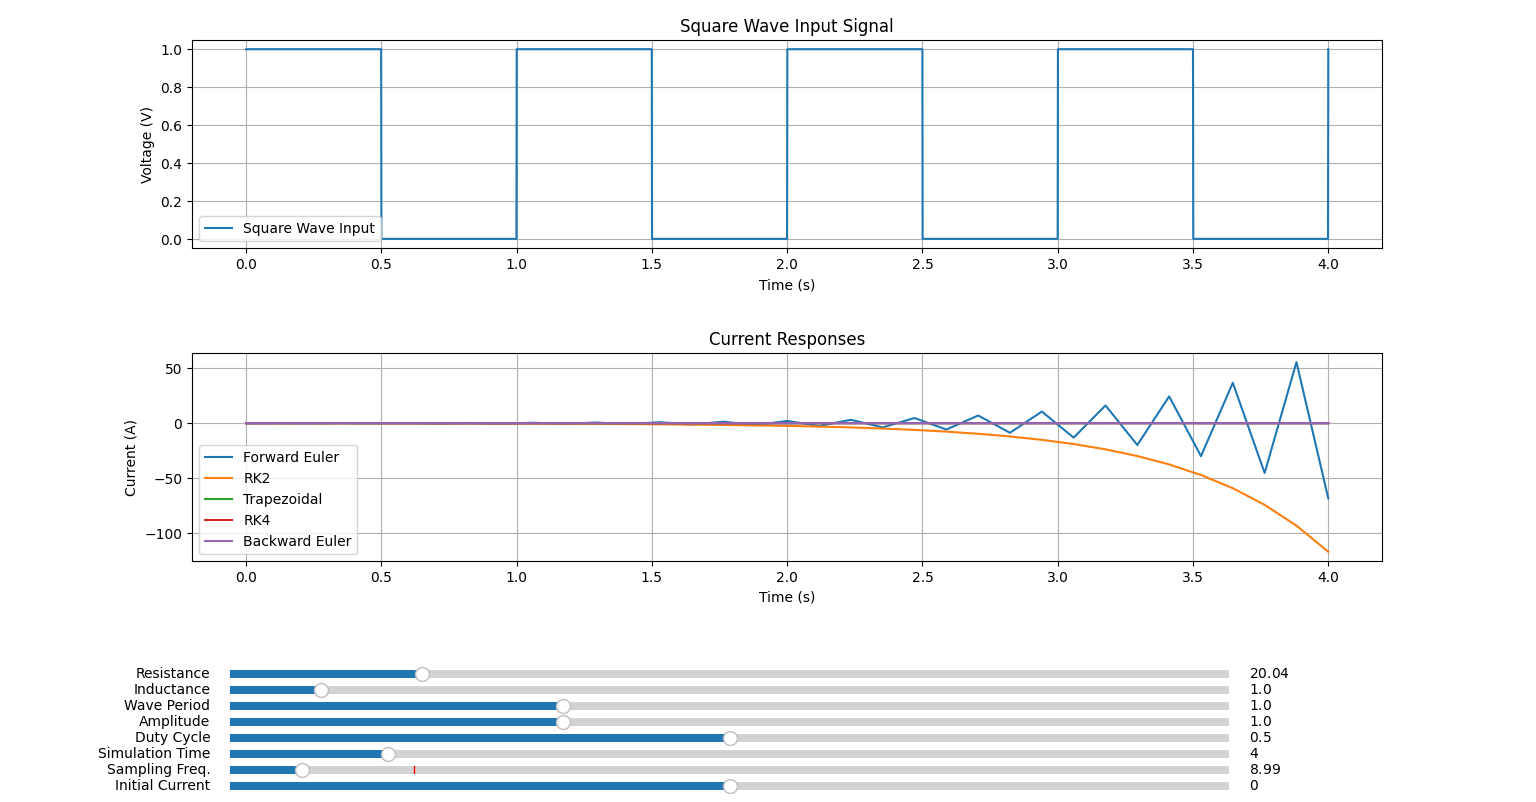
\includegraphics[width=\textwidth]{figs/instability_fwd_euler.png}
  \caption{Instability of the Forward Euler method for a step size that violates the stability condition.}
  \label{fig:instability_forward_euler}
\end{figure}

\subsection{Backward Euler Method}

\subsubsection*{General Algorithm}
The Backward Euler method is given by
\begin{align}
y_{n+1} &= y_n + h\, f(t_{n+1},y_{n+1}).
\end{align}

\subsubsection*{Geometric View}
Here the slope is taken at the new time level $(t_{n+1},y_{n+1})$, which improves stability by "looking ahead."

\subsubsection*{Derivation of Amplification Factor}
For the test equation $y'=\lambda y$, we have:
\begin{align}
y_{n+1} &= y_n + h\lambda y_{n+1}.
\end{align}
Rearranging,
\begin{align}
(1-h\lambda)y_{n+1} &= y_n, \\
y_{n+1} &= \frac{y_n}{1-h\lambda}.
\end{align}
Thus, the amplification factor is 
\begin{align}
R(z) &= \frac{1}{1-z}, \quad z=h\lambda.
\end{align}

\subsubsection*{Local Truncation Error}
A similar Taylor expansion argument shows that Backward Euler has an LTE of order $O(h)$.

\subsubsection*{Application to the RL Circuit}
For $\lambda=-\frac{R}{L}$, the Backward Euler update becomes 
\begin{align}
i_{n+1} &= i_n + h\left[-\frac{R}{L}\, i_{n+1}+\frac{V_{\text{in}}}{L}\right].
\end{align}

\subsection{Runge--Kutta 2nd Order (RK2) Method (Heun's Method)}
\subsubsection*{General Algorithm}
Heun's method is given by:
\begin{align}
k_1 &= f(t_n,y_n), \\
k_2 &= f(t_n+h, y_n+h\, k_1), \\
y_{n+1} &= y_n + \frac{h}{2}(k_1+k_2).
\end{align}

\subsubsection*{Geometric View}
This method first uses an Euler step to predict the solution at $t_n+h$, then uses the slope at that point to correct the estimate by averaging the two slopes.

\subsubsection*{Detailed Derivation and Amplification Factor}
For $y'=\lambda y$, we have:
\begin{align}
k_1 &= \lambda y_n, \\
y^p &= y_n + h\, k_1 = y_n(1+h\lambda), \\
k_2 &= \lambda y^p = \lambda y_n(1+h\lambda).
\end{align}
Thus, the update is:
\begin{align}
y_{n+1} &= y_n + \frac{h}{2}\left[\lambda y_n + \lambda y_n(1+h\lambda)\right] \\
         &= y_n\left[ 1 + h\lambda + \frac{(h\lambda)^2}{2} \right].
\end{align}
So, the amplification factor is 
\begin{align}
R(z) &= 1+z+\frac{z^2}{2}, \quad z=h\lambda.
\end{align}

\subsubsection*{Local Truncation Error}
Comparing with the exact solution $e^{h\lambda} = 1+h\lambda+\frac{(h\lambda)^2}{2}+\frac{(h\lambda)^3}{6}+\cdots$, the local error per step is 
\begin{align}
e^{h\lambda} - \left(1+h\lambda+\frac{(h\lambda)^2}{2}\right) &= \frac{(h\lambda)^3}{6}+O(h^4).
\end{align}
Thus, the LTE is $O(h^3)$ and when scaled by $h$, the method is second order accurate.

\subsubsection*{Application to the RL Circuit}
For the RL circuit,
\begin{align}
k_1 &= -\frac{R}{L}\, i_n+\frac{V_{\text{in}}}{L}, \\
k_2 &= -\frac{R}{L}\Bigl(i_n+h\, k_1\Bigr)+\frac{V_{\text{in}}}{L}, \\
i_{n+1} &= i_n + \frac{h}{2}(k_1+k_2).
\end{align}

\begin{figure}[htbp]
  \centering
  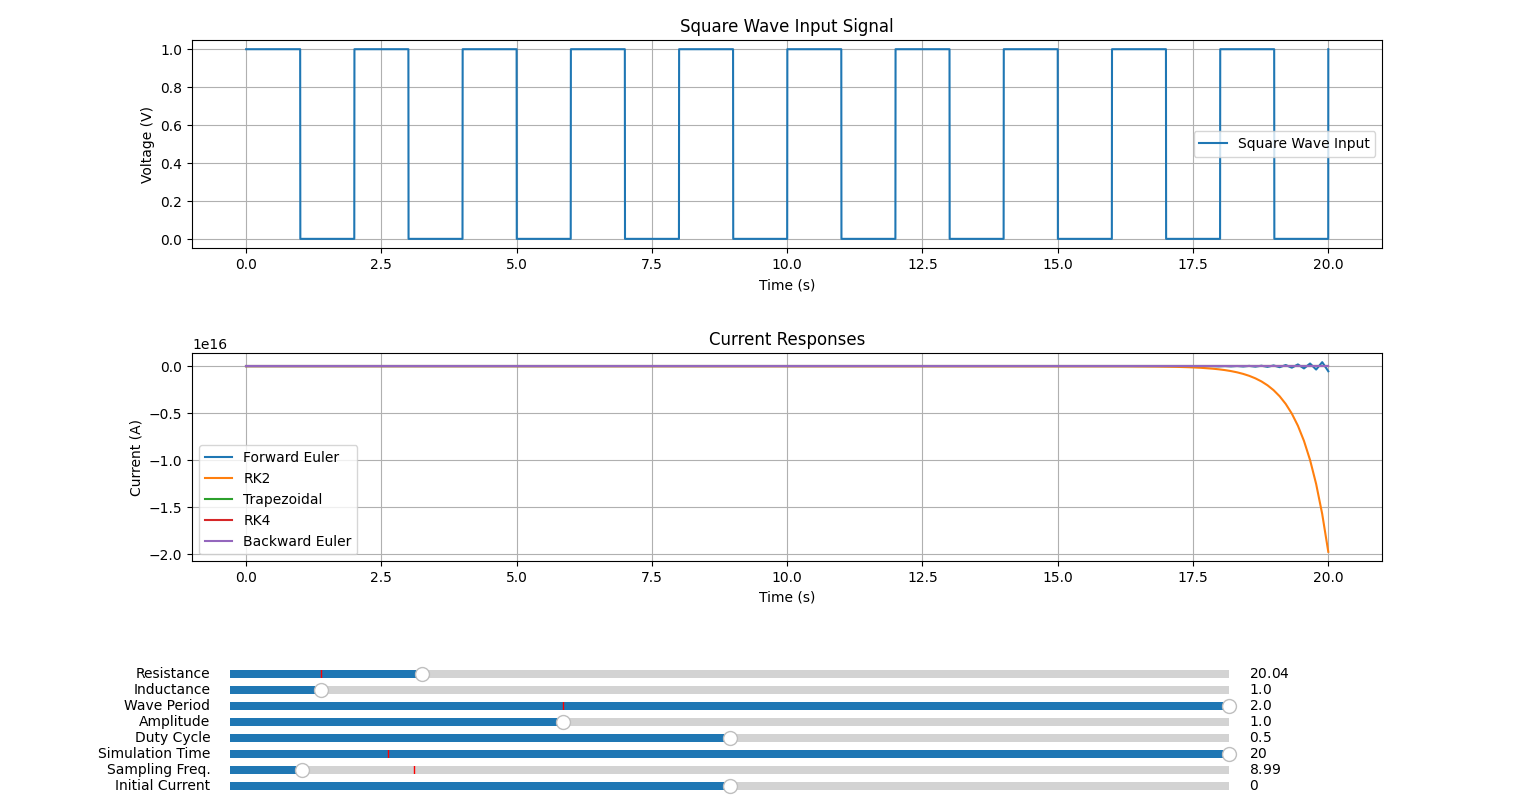
\includegraphics[width=\textwidth]{figs/instability_rk2.png}
  \caption{Instability behavior of RK2 (Heun's) method when the step size is too large.}
  \label{fig:instability_rk2}
\end{figure}

\subsection{Trapezoidal Method}

\subsubsection*{General Algorithm}
The Trapezoidal method is given by:
\begin{align}
y_{n+1} &= y_n + \frac{h}{2}\Bigl[f(t_n,y_n)+f(t_{n+1},y_{n+1})\Bigr].
\end{align}

\subsubsection*{Geometric View}
This method approximates the area under the curve by forming a trapezoid over the interval, averaging the slopes at the beginning and end of the step.

\subsubsection*{Derivation of Amplification Factor}
For $y'=\lambda y$, we substitute $f(t,y)=\lambda y$:
\begin{align}
y_{n+1} &= y_n + \frac{h\lambda}{2}(y_n+y_{n+1}).
\end{align}
Rearranging:
\begin{align}
y_{n+1}\left(1-\frac{h\lambda}{2}\right) &= y_n\left(1+\frac{h\lambda}{2}\right), \\
y_{n+1} &= \frac{1+\frac{h\lambda}{2}}{1-\frac{h\lambda}{2}}\, y_n.
\end{align}
Thus, the amplification factor is 
\begin{align}
R(z) &= \frac{1+\frac{z}{2}}{1-\frac{z}{2}}, \quad z=h\lambda.
\end{align}

\subsubsection*{Local Truncation Error}
A detailed derivation shows that the Trapezoidal method has an LTE of $O(h^3)$, implying it is second order accurate when scaled by $h$.

\subsubsection*{Application to the RL Circuit}
For the RL circuit, the update becomes:
\begin{align}
i_{n+1} &= i_n+\frac{h}{2}\Biggl[\left(-\frac{R}{L}\, i_n+\frac{V_{\text{in}}}{L}\right) + \left(-\frac{R}{L}\, i_{n+1}+\frac{V_{\text{in}}}{L}\right)\Biggr].
\end{align}
This implicit equation is solved for $i_{n+1}$.

\subsection{Runge--Kutta 4th Order (RK4) Method}

\subsubsection*{General Algorithm}
The RK4 method is defined by:
\begin{align}
k_1 &= f(t_n,y_n), \\
k_2 &= f\left(t_n+\frac{h}{2},\, y_n+\frac{h}{2}\,k_1\right), \\
k_3 &= f\left(t_n+\frac{h}{2},\, y_n+\frac{h}{2}\,k_2\right), \\
k_4 &= f(t_n+h,\, y_n+h\,k_3), \\
y_{n+1} &= y_n+\frac{h}{6}\Bigl(k_1+2k_2+2k_3+k_4\Bigr).
\end{align}

\subsubsection*{Geometric View}
RK4 evaluates the slope at four points (initial, two midpoints, and final) and computes a weighted average of these slopes to approximate the solution. This multi-stage process captures more information about the behavior of the solution over the interval.

\subsubsection*{Derivation of Amplification Factor}
For $y'=\lambda y$, the RK4 method’s amplification factor is given by the fourth-order Taylor polynomial of $e^{h\lambda}$:
\begin{align}
R(z) &= 1+z+\frac{z^2}{2}+\frac{z^3}{6}+\frac{z^4}{24}, \quad z=h\lambda.
\end{align}

\subsubsection*{Local Truncation Error}
The exact solution is 
\begin{align}
e^{h\lambda} &= 1+h\lambda+\frac{(h\lambda)^2}{2}+\frac{(h\lambda)^3}{6}+\frac{(h\lambda)^4}{24}+\frac{(h\lambda)^5}{120}+\cdots,
\end{align}
and the error per step is 
\begin{align}
e^{h\lambda} - R(z) &= \frac{(h\lambda)^5}{120}+O(h^6).
\end{align}
Thus, the LTE is $O(h^5)$, so when divided by $h$ the method is fourth order accurate.

\subsubsection*{Application to the RL Circuit}
For our circuit, with 
\[
f(i) = -\frac{R}{L}\, i + \frac{V_{\text{in}}}{L},
\]
the stages are:
\begin{align}
k_1 &= -\frac{R}{L}\, i_n + \frac{V_{\text{in}}}{L}, \\
k_2 &= -\frac{R}{L}\Bigl(i_n+\frac{h}{2}\, k_1\Bigr)+\frac{V_{\text{in}}}{L}, \\
k_3 &= -\frac{R}{L}\Bigl(i_n+\frac{h}{2}\, k_2\Bigr)+\frac{V_{\text{in}}}{L}, \\
k_4 &= -\frac{R}{L}\Bigl(i_n+h\, k_3\Bigr)+\frac{V_{\text{in}}}{L}, \\
i_{n+1} &= i_n+\frac{h}{6}\Bigl(k_1+2k_2+2k_3+k_4\Bigr).
\end{align}
The amplification factor for the homogeneous part remains 
\begin{align}
R(z) &= 1+z+\frac{z^2}{2}+\frac{z^3}{6}+\frac{z^4}{24}, \quad z=h\lambda.
\end{align}

\begin{figure}[htbp]
  \centering
  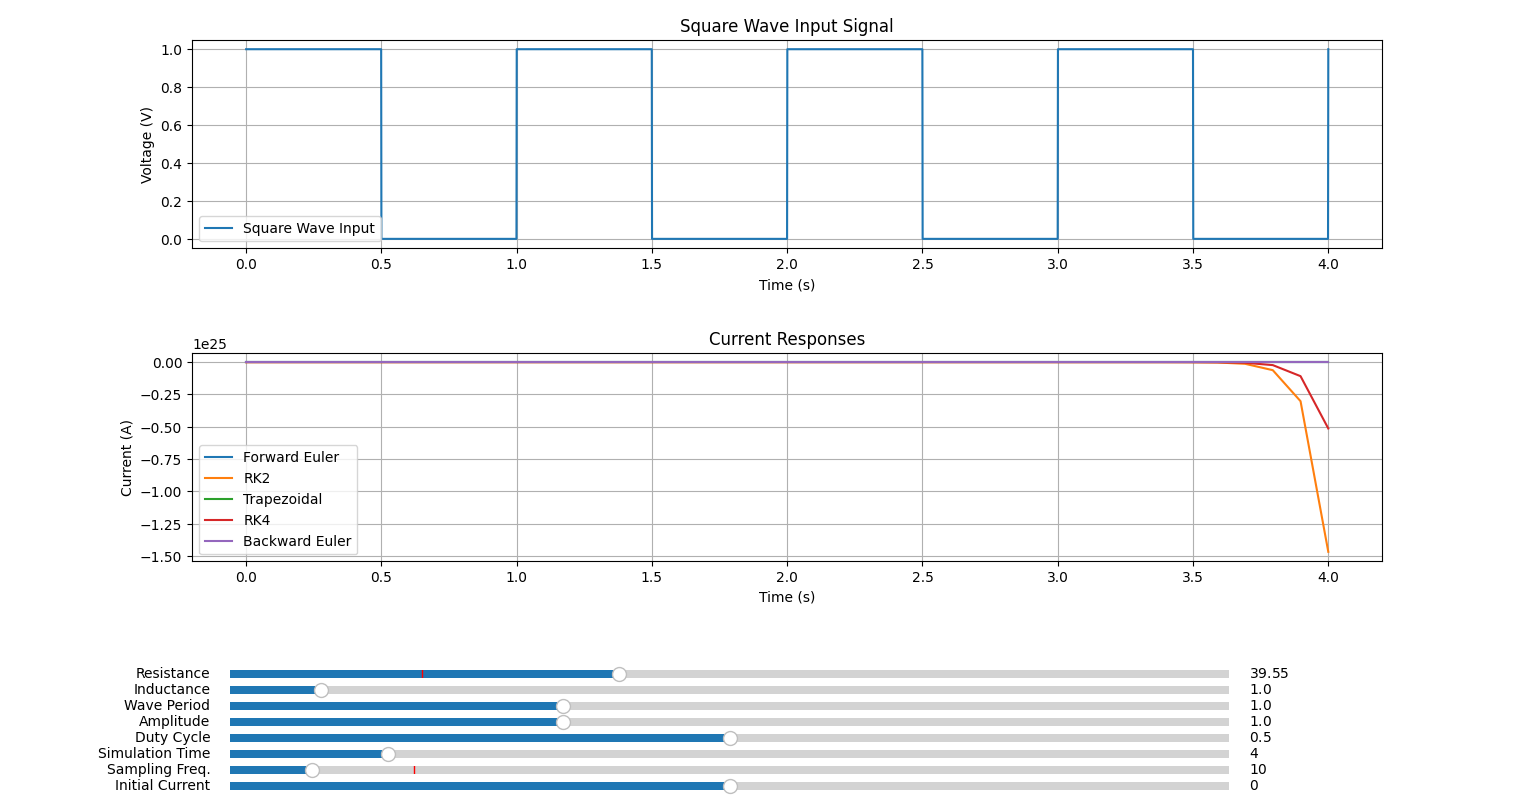
\includegraphics[width=\textwidth]{figs/instability_rk4.png}
  \caption{Instability behavior of RK4 when the step size exceeds the stability region (bounded region).}
  \label{fig:instability_rk4}
\end{figure}

\section{Error Comparison and Reference Method}
In this section, we compare the performance of the various numerical methods by plotting their local and global errors. Figure~\ref{fig:local_error} shows the local truncation error at each sample point for selected values of $R$, $L$, and the sampling rate. In Figure~\ref{fig:global_error}, the global error of the methods is plotted against the sampling factor, with the RK4 method used as the reference.

RK4 was chosen as the reference method because its higher order accuracy (with a global error of order $O(h^4)$) ensures that its error is significantly smaller than that of lower-order methods. This makes it a reliable benchmark for comparing the performance and error behavior of other numerical schemes.

\begin{figure}[htbp]
  \centering
  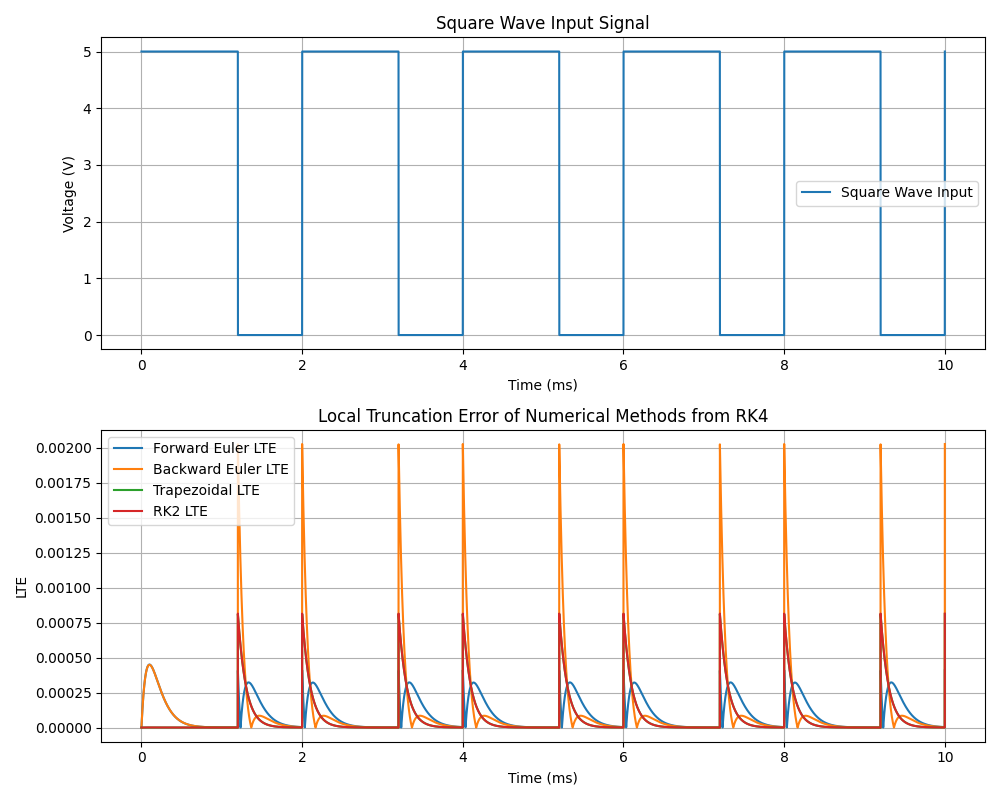
\includegraphics[width=\textwidth]{figs/local_error.png}
  \caption{Local truncation error at each sample point for selected values of $R$, $L$, and the sampling rate.}
  \label{fig:local_error}
\end{figure}

\begin{figure}[htbp]
  \centering
  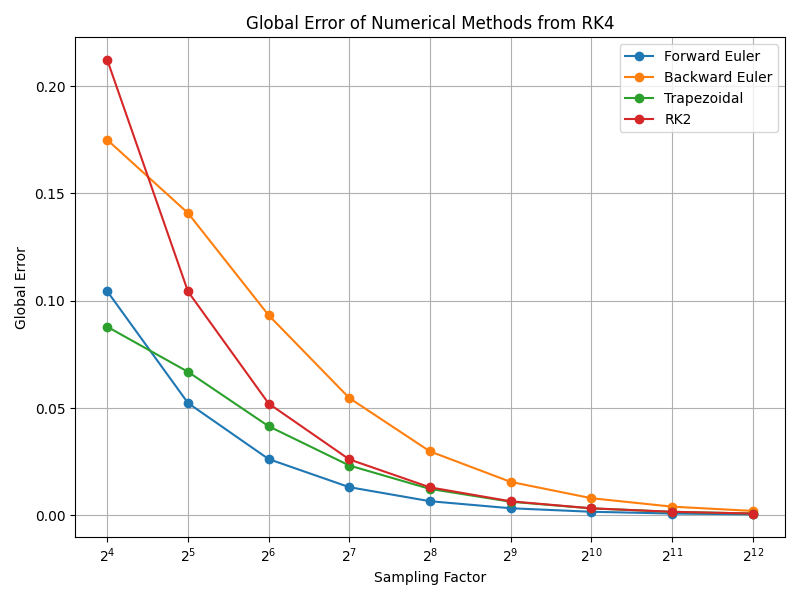
\includegraphics[width=\textwidth]{figs/global_error.png}
  \caption{Global error versus the sampling factor. The RK4 method is used as the reference due to its higher order accuracy ($O(h^4)$).}
  \label{fig:global_error}
\end{figure}

\section{Computational Times Comparison}
Figure~\ref{fig:comp_times} plots the computational times (y-axis) versus the sampling factors (x-axis) for the different methods. This comparison helps illustrate the trade-off between accuracy, stability, and computational cost. As the sampling factor increases (i.e., as $h$ decreases), the computational time typically increases. 

\begin{figure}[htbp]
  \centering
  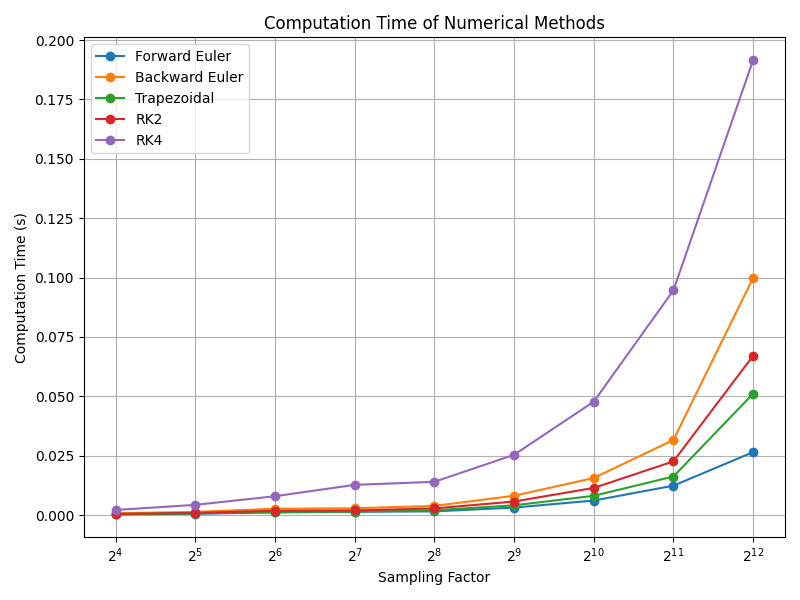
\includegraphics[width=\textwidth]{figs/computation_time.png}
  \caption{Computational times (y-axis) versus sampling factors (x-axis) for the different methods.}
  \label{fig:comp_times}
\end{figure}

\section{Stability Analysis Summary}
For a one-step method applied to the test equation 
\begin{align}
y' &= \lambda y, \quad y(0)=y_0,
\end{align}
the update can be written as 
\begin{align}
y_{n+1} &= R(z)y_n, \quad \text{with } z = h\lambda.
\end{align}
A method is stable if 
\begin{align}
|R(z)| &< 1.
\end{align}
For the RL circuit, the homogeneous part is 
\begin{align}
\frac{di}{dt} &= -\frac{R}{L}\, i,
\end{align}
so $\lambda=-\frac{R}{L}$. Each method’s amplification factor $R(z)$ then determines the choice of $h$ to ensure stability:
\begin{itemize}
    \item \textbf{Forward Euler:} $R(z)=1+z$ $\Rightarrow$ requires $\left|1-h\frac{R}{L}\right|<1$.
    \item \textbf{Backward Euler:} $R(z)=\frac{1}{1-z}$ is A-stable.
    \item \textbf{RK2 (Heun's):} $R(z)=1+z+\frac{z^2}{2}$.
    \item \textbf{Trapezoidal:} $R(z)=\frac{1+\frac{z}{2}}{1-\frac{z}{2}}$ is A-stable.
    \item \textbf{RK4:} $R(z)=1+z+\frac{z^2}{2}+\frac{z^3}{6}+\frac{z^4}{24}$ has a bounded stability region.
\end{itemize}

\section{Conclusion}
In this report, we have reviewed five numerical methods for solving ODEs and derived their amplification factors and local truncation errors step by step using the test equation $y'=\lambda y$. For our project, we apply these methods to a series RL circuit described by 
\begin{align}
L\frac{di}{dt}+Ri &= V_{\text{in}},
\end{align}
or equivalently,
\begin{align}
\frac{di}{dt} &= -\frac{R}{L}\, i + \frac{V_{\text{in}}}{L}.
\end{align}
The methods are summarized below in the context of the RL circuit:
\begin{itemize}
    \item \textbf{Forward Euler:} 
    \begin{align}
    i_{n+1} &= i_n+h\left[-\frac{R}{L}\, i_n+\frac{V_{\text{in}}}{L}\right],
    \end{align}
    with LTE of $O(h)$.
    \item \textbf{Backward Euler:} 
    \begin{align}
    i_{n+1} &= i_n+h\left[-\frac{R}{L}\, i_{n+1}+\frac{V_{\text{in}}}{L}\right],
    \end{align}
    with LTE of $O(h)$.
    \item \textbf{RK2 (Heun's Method):} 
    \begin{align}
    k_1 &= -\frac{R}{L}\, i_n+\frac{V_{\text{in}}}{L}, \\
    k_2 &= -\frac{R}{L}\Bigl(i_n+h\, k_1\Bigr)+\frac{V_{\text{in}}}{L}, \\
    i_{n+1} &= i_n+\frac{h}{2}(k_1+k_2),
    \end{align}
    with LTE of $O(h^3)$ (i.e., second order accurate).
    \item \textbf{Trapezoidal:} 
    \begin{align}
    i_{n+1} &= i_n+\frac{h}{2}\Biggl[\left(-\frac{R}{L}\, i_n+\frac{V_{\text{in}}}{L}\right)+\left(-\frac{R}{L}\, i_{n+1}+\frac{V_{\text{in}}}{L}\right)\Biggr],
    \end{align}
    with LTE of $O(h^3)$.
    \item \textbf{RK4:} 
    \begin{align}
    k_1 &= -\frac{R}{L}\, i_n+\frac{V_{\text{in}}}{L}, \\
    k_2 &= -\frac{R}{L}\Bigl(i_n+\frac{h}{2}\, k_1\Bigr)+\frac{V_{\text{in}}}{L}, \\
    k_3 &= -\frac{R}{L}\Bigl(i_n+\frac{h}{2}\, k_2\Bigr)+\frac{V_{\text{in}}}{L}, \\
    k_4 &= -\frac{R}{L}\Bigl(i_n+h\, k_3\Bigr)+\frac{V_{\text{in}}}{L}, \\
    i_{n+1} &= i_n+\frac{h}{6}\Bigl(k_1+2k_2+2k_3+k_4\Bigr),
    \end{align}
    with LTE of $O(h^5)$ (i.e., fourth order accurate).
\end{itemize}
The choice among these methods depends on the circuit parameters, the required accuracy, and the stiffness of the problem. For non-stiff conditions, RK4 may be preferred for its high accuracy, while for stiff transients the implicit methods (Backward Euler or Trapezoidal) are more appropriate.

\end{document}
